% command to make sure colorboxes don't create whitespace between code lines
\fboxsep=.6pt

% default settings for listings
\lstset{style=python, basicstyle=\ttfamily\footnotesize}

\title[Programmieren]{Programmieren: Klassen}

\subtitle{Klassen}

\author[Wendl, Cyril] % (optional)
{Cyril Wendl}

\institute[KLW] % (optional)
{
	Fachschaft Informatik\\
	Kantonsschule im Lee
}

\date[\today] % (optional)

\logo{
\includegraphics[width=2cm]{Logos/LeeLogo}}

\titlegraphic{\vspace{-.7cm}\includegraphics[width=\textwidth]{"Grundlagen_Info/06_Datenbanken/Figures/title-emojis"}}

\frame{\titlepage}

\begin{frame}[fragile]{Klassen in Python}
	\begin{figure}[H]
		\begin{tikzpicture}[font=\sffamily\footnotesize, scale=.6]
			% Styles
			\tikzset{
				title/.style={align=center},
				col/.style={align=left, text width=4.5cm}
			}

			% --- Links: Klasse Hund (Bauplan) ---
			\node[inner sep=0pt] (dogclass) at (1.8,2.6)
			{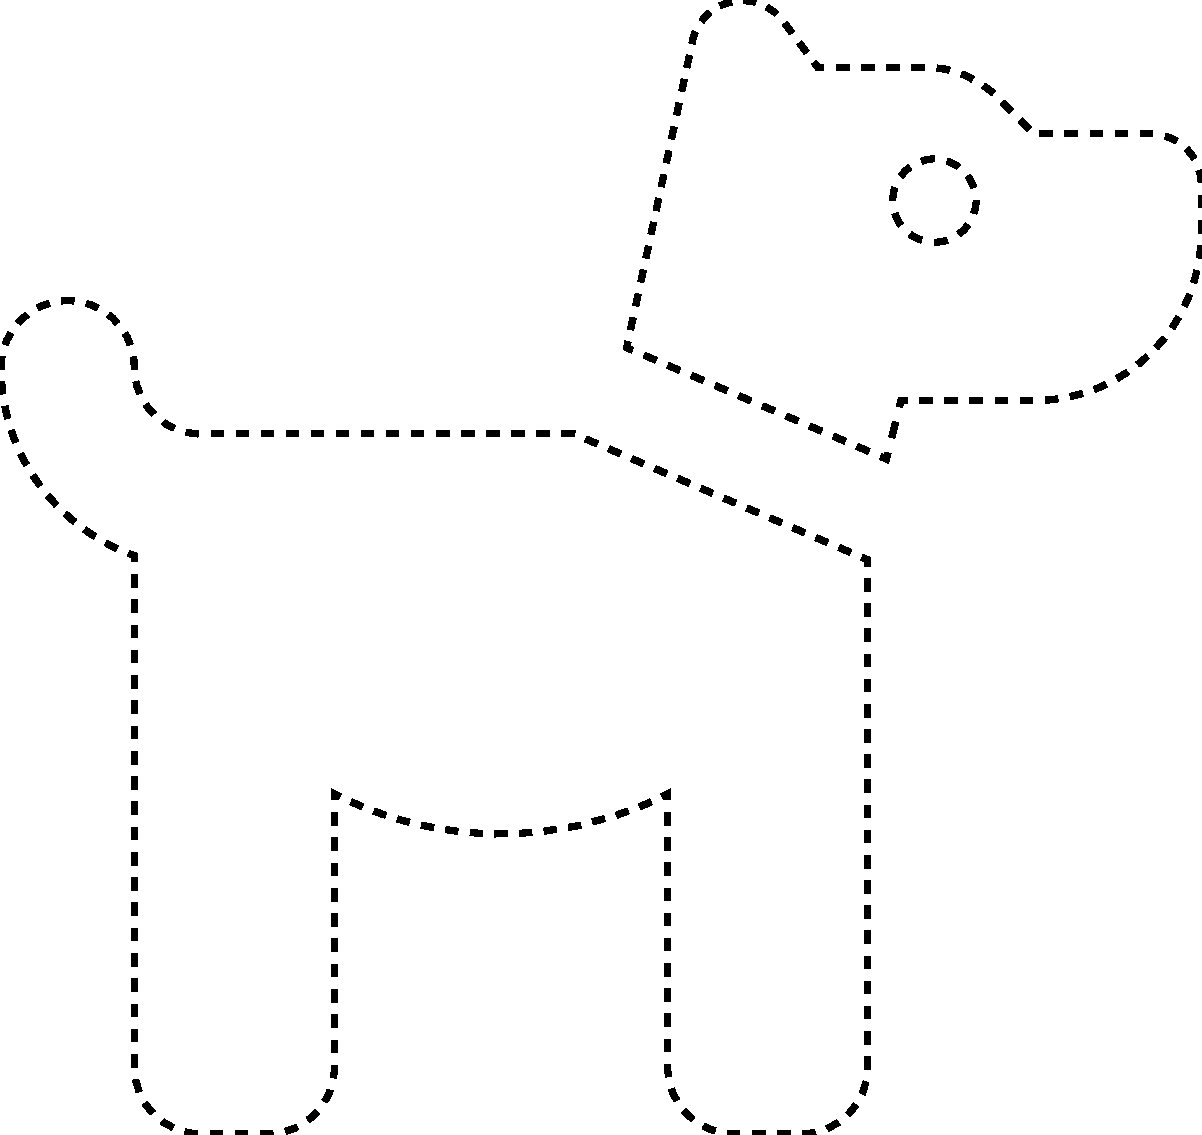
\includegraphics[width=2.5cm]{Grundlagen_Info/00_Programmieren/Skript/Figures/dog-class.pdf}};
			% --- Rechts: mehrere Instanzen gestapelt ---
			% Basisinstanz
			\onslide<2->{
				\node[inner sep=0pt] (dog1) at (10.0,2.6)
				{
\includegraphics[width=2.5cm]{Grundlagen_Info/00_Programmieren/Skript/Figures/dog-instance1.pdf}};
			}
			% Überlagerungen leicht verschoben
			\onslide<3->{\node[inner sep=0pt, anchor=south west] at ($(dog1.south west)+(0.3,0.3)$)
				{
\includegraphics[width=2.5cm]{Grundlagen_Info/00_Programmieren/Skript/Figures/dog-instance2.pdf}};}
			\onslide<4->{

				\node[inner sep=0pt, anchor=south west] at ($(dog1.south west)+(0.6,0.6)$)
				{
\includegraphics[width=2.5cm]{Grundlagen_Info/00_Programmieren/Skript/Figures/dog-instance3.pdf}};}

			\node[title, above=0.5cm of dogclass] {Klasse};
			\node[align=center,text width=4.5cm, font=\small, below=0.2cm of dogclass] {\lstinline|class Hund:|};
			\onslide<5->{
				\node[title, above=0.5cm of dog1] {Objekte / Instanzen};}

			% Pfeil
			\onslide<2->{\draw[-Latex, thick] (dogclass.east) -- node[above]{Instanz(en) erzeugen} (dog1.west);}
		\end{tikzpicture}
	\end{figure}
	\pause
	\begin{lstlisting}
		hund1 = Hund("Thommy", 510, "Grün")
		hund2 = Hund("Bello", 380, "Gelb")
		hund3 = Hund("Rocky", 315, "Rot")
		# ...
		\end{lstlisting}
	\begin{itemize}
		\item<6-> Eigenschaften / Attribute: \lstinline|name|, \lstinline|farbe|, \lstinline|alter|, etc.
		\item<7-> Methoden: \lstinline|.bellen()|, \lstinline|.sitzen()|, etc.
		\item<8-> \textbf{Wird in Games ständig verwendet, um Objekte zu \enquote{spawnen}!}
	\end{itemize}

\end{frame}

\begin{frame}{Klassen in Python}
	\begin{itemize}[<+->]
		\item Eine Klasse ist ein Bauplan für Objekte.
		\item Sie definiert Eigenschaften (Attribute) und Verhalten (Methoden) von Objekten.
		\item Klassen ermöglichen die Erstellung von benutzerdefinierten Datentypen.
		\item 
		Wir kennen Klassen bereits von anderen Typen: \textbf{Listen, Zahlen, Zeichenketten!}
	\end{itemize}
	

\end{frame}

\begin{frame}[fragile]{Listen als Klassen}
	\begin{figure}[H]
		\begin{tikzpicture}[font=\sffamily\footnotesize, scale=0.6]
			% Styles
			\tikzset{
				title/.style={align=center},
				col/.style={align=left, text width=4.5cm}
			}

			% --- Links: Klasse Liste (Bauplan) ---
			% --- Links: Klasse Liste (Bauplan) ---
			% Draw dashed circle
			\draw[dashed, thick] (1.8,2.6) circle [radius=0.5cm];
			% Icon node inside circle
			\node[inner sep=0pt] (listclass) at (1.8,2.6)
			{\faListUl}; % FontAwesome list icon for class

			% --- Rechts: mehrere Instanzen als Icons ---
			\node[inner sep=0pt] (list1) at (10.0,2.4)
			{\textcolor{Crimson}{\faListUl}}; % FontAwesome square icon for instance
			\node[inner sep=0pt] at (10.5,2.6)
			{\textcolor{RoyalBlue}{\faListUl}};
			\node[inner sep=0pt] at (11,2.8)
			{\textcolor{ForestGreen}{\faListUl}};

			\node[title, above=0.7cm of listclass] {Klasse};
			\node[align=center,text width=4.5cm, font=\small, below=0.4cm of listclass] {\lstinline|class list:|};
			\node[title, above=0.7cm of list1] {Objekte / Instanzen};
			\node[align=center,text width=4.5cm, font=\small, below=0.4cm of list1] {\begin{lstlisting}
	liste1 = [1,2,3]
	liste2 = ["a","b"]
	liste3 = [True, False]
	# ...
	\end{lstlisting}};

			% Pfeil
			\draw[-Latex, thick] (2.2,2.6) -- node[above]{Instanz(en) erzeugen} (9.6, 2.6);

			% Linke Spalten
			\node[anchor=west, col] at (-2.0,-3.5) {\textbf{Attribute}\\
				\texttt{Elemente}\\
				\texttt{Länge}\\
				...};

			\node[anchor=west, col] at (2.4,-3.5) {\textbf{Methoden}\\
				\texttt{append()}\\
				\texttt{remove()}\\
				\texttt{sort()}\\
				\texttt{pop()}\\
				\texttt{count()}\\
				...};

			% Rechte Spalten
			\node[anchor=west, col] at (6.2,-3.5) {\textbf{Attribute}\\
			\texttt{Elemente : [1,2,3]}\\
			\texttt{Länge : 3}\\
			...};

			\node[anchor=west, col] at (11.9,-3.5) {\textbf{Methoden}\\
				\texttt{append()}\\
				\texttt{remove()}\\
				\texttt{sort()}\\
				\texttt{pop()}\\
				\texttt{count()}\\
				...};

		\end{tikzpicture}
	\end{figure}
\end{frame}

\setbeamertemplate{logo}{} % Hide logo
\begin{frame}[fragile]{Beispiel: Personen}
	\begin{lstlisting}[basicstyle=\ttfamily\scriptsize, escapechar=!, numbers=left,framerule=1pt]
class Person:
    def __init__(self, name, alter):!\tikzmark{initStart}!                                
        self.name = name
        self.alter = alter         !\tikzmark{initEnd}!
    
    def vorstellen(self):!\tikzmark{method1Start}!                !\tikzmark{method1Comment}!
        print(f"Hallo, ich bin {self.name} und {self.alter} Jahre alt.")
		
	def geburtstag_feiern(self):!\tikzmark{method2Start}!         !\tikzmark{method2Comment}!
        self.alter += 1
        print(f"{self.name} ist jetzt {self.alter} Jahre alt.")

    

# Objekte der Klasse Person erstellen
anna = Person("Anna", 16)
jan = Person("Jan", 17)

# Methoden aufrufen
anna.vorstellen()  # Ausgabe: Hallo, ich bin Anna und 16 Jahre alt.
jan.vorstellen()   # Ausgabe: Hallo, ich bin Jan und 17 Jahre alt.

# Geburtstag feiern
anna.geburtstag_feiern()  # Ausgabe: Anna ist jetzt 17 Jahre alt.
\end{lstlisting}
	\begin{tikzpicture}[overlay, remember picture,
			every node/.style={draw=red!50,fill=red!50!white,text=black,rounded corners}]
		\only<2->{\drawBrace{1em}{initStart}{initEnd}{\makecell{\footnotesize Instanzen erstellen\\\footnotesize (initialisieren)}}{.5}{}{3em};}
		\only<3->{\drawArrow{method1Start}{method1Comment}{\footnotesize Methode}{RoyalBlue!50!white};}
		\only<4->{\drawArrow{method2Start}{method2Comment}{\footnotesize Methode}{RoyalBlue!50!white};}

	\end{tikzpicture}
	\footnotesize\textbf{\lstinline|class ...| ist der Klassenname, \lstinline|self| bezieht sich auf die aktuelle Instanz.}
\end{frame}
\setbeamertemplate{logo}{
\includegraphics[width=2cm]{Logos/LeeLogo}}


\begin{frame}[fragile]{Aufgaben}{Programmier-Skript}
	\begin{itemize}
		\item \readbox{Definition 7.1, Beispiele 7.1-7.2} \\[.3cm]
$\rightarrow$ Ausführen und zwei weitere Instanzen von \lstinline|Person| erstellen.
		\item \aufgabebox{Aufgaben 7.1, 7.2} $\rightarrow$ Zuerst auf VS Code, dann Test auf Moodle
		\item Schnelle: \aufgabebox{Aufgabe 7.3, 7.4} (Skript selber lesen)
	\end{itemize}
\end{frame}

\begin{frame}[fragile]{Zusammenfassung: Klassen}
	\begin{itemize}[<+->]
		\item Klasse = eine Art von Variable
		\item \textbf{Variable} = eine Instanz der Klasse
		\item Z.B. \lstinline|meineliste=[10,6,1]| $\Rightarrow$ \lstinline|list| (Instanz der Klasse \lstinline|list|)
		\item Klassen können \textbf{Attribute} und \textbf{Methoden} haben: z.B. \lstinline|hund = Hund("Bello", 3)| $\Rightarrow$ \lstinline|hund.name| (Attribut) und \lstinline|hund.bellen()| (Methode)
	\end{itemize}
\end{frame}